%% IEEE Transactions on Information Theory -- single-column review manuscript.
%% Draft prepared August 2026.
\documentclass[letterpaper,onecolumn]{IEEEtran}

\usepackage[T1]{fontenc}
\usepackage[utf8]{inputenc}
\usepackage{amsmath,amssymb,amsthm,mathtools}
\usepackage{booktabs}
\usepackage{array}
\usepackage{bm}
\usepackage{microtype}
\usepackage{cite}
\usepackage{xcolor}
\usepackage{flafter}
\usepackage{tikz}
\usetikzlibrary{arrows.meta,positioning,calc,fit,backgrounds}
\usepackage{pgfplots}
\pgfplotsset{compat=1.18}
\usepackage[colorlinks=true,linkcolor=blue,citecolor=blue,urlcolor=blue]{hyperref}
\hypersetup{pdftitle={A Rate--Work--Distortion Region for Consumer-Relative Observation},pdfauthor={Andrew H. Bond}}

\newtheorem{theorem}{Theorem}
\newtheorem{proposition}{Proposition}
\newtheorem{lemma}{Lemma}
\newtheorem{corollary}{Corollary}
\theoremstyle{definition}
\newtheorem{definition}{Definition}
\newtheorem{example}{Example}
\theoremstyle{remark}
\newtheorem{remark}{Remark}

\newcommand{\E}{\mathbb{E}}
\newcommand{\R}{\mathbb{R}}
\newcommand{\cC}{\mathcal{C}}
\newcommand{\cX}{\mathcal{X}}
\newcommand{\hX}{\widehat{X}}
\newcommand{\hXn}{\widehat{X}^{n}}
\newcommand{\RW}{\mathcal{R}\!\mathcal{W}}
\newcommand{\PC}{P_{\mathcal{C}}}
\newcommand{\tr}{\operatorname{tr}}
\newcommand{\diag}{\operatorname{diag}}
\newcommand{\rank}{\operatorname{rank}}
\newcommand{\clconv}{\overline{\operatorname{conv}}}
\newcommand{\1}{\mathbf{1}}
\newcommand{\kb}{k_{\mathrm B}}
\newcommand{\hbin}{h_2}

\begin{document}

\title{A Rate--Work--Distortion Region for\\Consumer-Relative Observation}

\author{Andrew~H.~Bond,~\IEEEmembership{Senior~Member,~IEEE}%
\thanks{Draft prepared August 2026. The author is with the Department of
Computer Engineering, San Jos\'e State University, San Jos\'e, CA 95192 USA
(e-mail: andrew.bond@sjsu.edu; ORCID 0009-0003-2599-6158).}%
\thanks{This manuscript develops the thermodynamic extension of the author's
Observation Theory program. The companion manuscript and reproducibility
materials are available at \url{https://github.com/ahb-sjsu/geometric-observation}.}}

\markboth{IEEE TRANSACTIONS ON INFORMATION THEORY (DRAFT)}%
{BOND: A RATE--WORK--DISTORTION REGION}

\maketitle

\begin{abstract}
Source coding counts the bits needed to serve a consumer. A cyclic physical
observer must also erase the memory that carried those bits. The two costs
coincide only when no correlated side information survives at reset. We study
a memory that stores a lossy description of an i.i.d. source, supports a
declared consumer distortion without access to side information, and is later
erased while correlated side information is retained. Under the classical,
isothermal Landauer model, we characterize the complete achievable region of
description rate, ideal reset work, and consumer distortion. For a test channel
from the source to its reconstruction, the two coordinates are the ordinary
mutual information and the mutual information conditioned on the reset side
information. The work-only endpoint is the common-reconstruction
rate--distortion function, but the full two-resource region distinguishes codes
that have the same rate and distortion and different thermodynamic costs. We
derive the supporting-channel equations for its Pareto boundary and give an
exact binary example with a nontrivial rate--work frontier. We then prove a
materialize-then-project barrier: once a full digital source record has been
created, jointly resetting it and every derived description costs its full
conditional entropy, regardless of the consumer's lower-dimensional need. We
extend the region to several consumers, identify the conditional total
correlation saved by coordinated reset, derive the Landauer scaling of the
Gaussian read-operator water-filling solution, and obtain a temperature-weighted
water-filling rule for heterogeneous memory banks. With jointly Gaussian reset
side information, the scalar region collapses to a single corner whose
rate--work gap grows to the full source--side-information mutual information as
distortion vanishes, while the vector frontier reappears as a generalized
water-filling in which the minimum-rate and minimum-work allocations differ.
Finally, for a stale Markov
record, predictive information lost with age is gained exactly as conditional
erasure work. The results concern the reversible lower bound on reset work, not
the total energy of sensing, communication, or finite-time operation.
\end{abstract}

\begin{IEEEkeywords}
Common reconstruction, consumer-relative distortion, information
thermodynamics, Landauer principle, rate--distortion theory, semantic source
coding, side information, source coding, thermodynamics of information.
\end{IEEEkeywords}

\IEEEpeerreviewmaketitle

\section{Introduction}\label{sec:intro}

Source coding asks how many bits a consumer needs. A cyclic physical observer
has a second obligation: it must eventually clear the memory that carried those
bits. Landauer's principle assigns a thermodynamic cost to this logically
irreversible step \cite{landauer1961,bennett1973}. In the ideal classical model,
erasing one unbiased bit from a symmetric memory coupled to a bath at
temperature $T$ requires at least $\kb T\ln 2$ of work. If correlated side
information remains available, the relevant quantity is conditional entropy
rather than entropy \cite{delrio2011,faist2015}. Thus a description can be
expensive to communicate and cheap to erase, or the reverse.

This paper studies that separation. A source block $X^n$ is encoded into a
memory index $M$. A consumer reconstructs $\hXn$ from $M$ alone and is judged by
a declared distortion $d_{\cC}$. Later, when $M$ is reset, a correlated block
$S^n$ is available to the reset mechanism. The consumer never sees $S^n$.
Figure~\ref{fig:model} shows the distinction. The rate of the description is
controlled by the size of $M$; its ideal reset work is controlled by
$H(M\mid S^n)$.

\begin{figure}[!t]
\centering
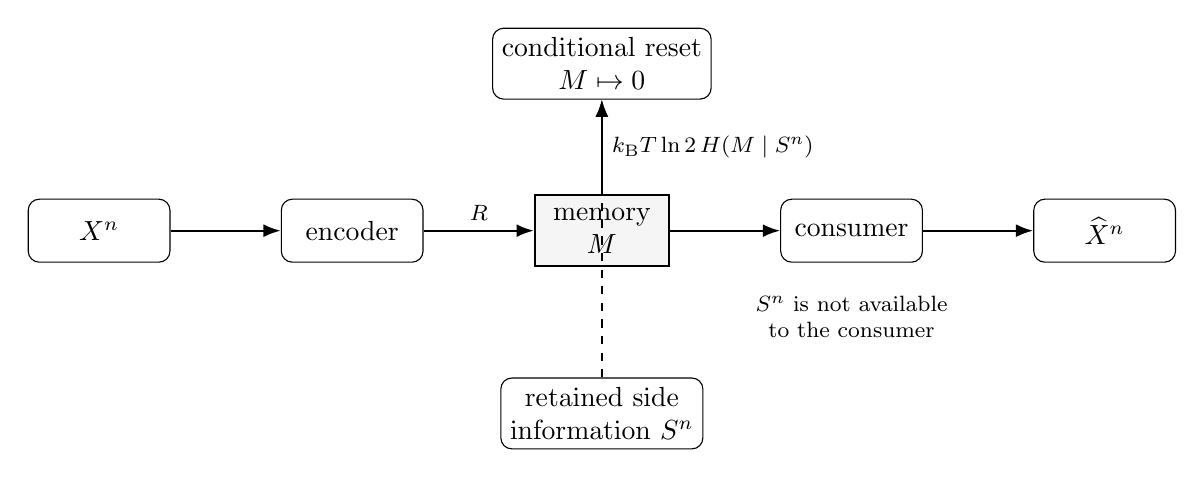
\begin{tikzpicture}[
  node distance=12mm and 14mm,
  block/.style={draw,rounded corners,minimum height=8mm,minimum width=18mm,align=center},
  mem/.style={draw,thick,minimum height=9mm,minimum width=17mm,align=center,fill=gray!8},
  arr/.style={-{Latex[length=2.2mm]},thick},
  darr/.style={-{Latex[length=2.2mm]},thick,dashed}
]
  \node[block] (x) {$X^n$};
  \node[block,right=of x] (enc) {encoder};
  \node[mem,right=of enc] (m) {memory\\$M$};
  \node[block,right=of m] (dec) {consumer};
  \node[block,right=of dec] (xh) {$\widehat X^n$};
  \node[block,below=14mm of m] (s) {retained side\\information $S^n$};
  \node[block,above=12mm of m] (rst) {conditional reset\\$M\mapsto 0$};
  \draw[arr] (x)--(enc);
  \draw[arr] (enc)--node[above,font=\footnotesize]{$R$}(m);
  \draw[arr] (m)--(dec);
  \draw[arr] (dec)--(xh);
  \draw[darr] (s)--(rst);
  \draw[arr] (m)--node[right,font=\footnotesize]{$\kb T\ln2\,H(M\mid S^n)$}(rst);
  \node[font=\footnotesize,align=center,below=3mm of dec] {$S^n$ is not available\\to the consumer};
\end{tikzpicture}
\caption{The model. The consumer reconstructs from the stored description alone.
Correlated side information is available only when the description memory is
reset. Rate and reset work are therefore different resources.}
\label{fig:model}
\end{figure}

The distortion is consumer-relative. Let $\cC$ be the map that reads an
observation and let $D_{\mathcal Y}$ be the loss on its output. The induced
distortion may be written
\begin{equation}
 d_{\cC}(x,\hat x)
   =D_{\mathcal Y}\!\left(\cC(x),\cC(\hat x)\right).
 \label{eq:consumer-dist}
\end{equation}
This is the exact form used in Observation Theory \cite{bond2026observation}.
Ordinary reconstruction is the special case in which $\cC$ is the identity and
$D_{\mathcal Y}$ is a source-space metric. The present paper takes
$d_{\cC}$ as given and asks a different question: what thermodynamic work is
forced by a representation that meets it?

The main result is a rate--work--distortion region. For each test channel
$p(\hat x\mid x)$ meeting the distortion constraint, the description-rate
coordinate is $I(X;\hX)$ and the normalized reset-work coordinate is
$I(X;\hX\mid S)$. Their separate minima do not, in general, describe the full
frontier: two test channels can have the same rate and distortion but different
conditional work. The work-only endpoint coincides mathematically with the
common-reconstruction rate--distortion function of Steinberg
\cite{steinberg2009}. That connection is useful rather than accidental. In the
common-reconstruction problem, side information reduces a communication rate
while the reconstruction remains reproducible without it. Here the same
conditional mutual information measures work saved when side information is
available only at erasure. The full region keeps the ordinary description rate
and the conditional reset work as distinct coordinates. This distinction is
also related to the classical separation between fixed-rate and
entropy-constrained quantization \cite{chou1989,chou1990}; the new ingredient is
that the entropy coordinate is conditional on information retained by the reset
mechanism and is assigned a thermodynamic meaning.

Six consequences follow. First, the lower boundary has a direct
supporting-channel characterization, and even a two-bit source exhibits a
strict tradeoff between description capacity and reset work. Second, a full
digital record cannot be made thermodynamically cheap by compressing it after
the fact. If a register holding
$X^n$ has already been materialized, the ideal work required to reset that
register and every deterministic description derived from it is
$\kb T\ln2\,H(X^n\mid S^n)$. Consumer-native observation saves work only when
irrelevant distinctions are never committed to volatile memory, or are
reversibly uncomputed. Third, a shared observation for several consumers is
priced by the joint consumer output; coordinated reset saves their conditional
total correlation. Fourth, for a Gaussian source and the read operator
$\PC$ of Observation Theory, the usual spectral water-filling rate becomes an
isothermal work law. If eigenmodes are erased in memory banks at different
temperatures, the water level is proportional to temperature. Fifth, with
jointly Gaussian reset side information the scalar region is a single corner
whose rate--work gap grows to $I(X;S)$ as distortion vanishes, and the
tradeoff reappears in the vector case through the allocation of distortion
across modes that the reset context knows unequally well. Sixth, for a
stale Markov record, the loss of predictive information and the rise of
conditional reset work are two sides of the same entropy identity.

The physical scope is deliberately narrow. We count the reversible lower bound
for resetting a classical, degenerate memory in the asymptotic i.i.d. regime.
We do not claim that sensing, transmitting, or switching a bit costs exactly
$\kb T\ln2$. Real devices operate far above the Landauer scale, finite-time
operation adds dissipation, and nondegenerate or quantum memories require more
general free-energy and one-shot treatments
\cite{sagawa2009,reeb2014,faist2015}. The point is not a present-day power model.
It is to identify which distinctions must be physically instantiated before
engineering losses are added.

\section{Model and physical accounting}\label{sec:model}

All logarithms are base two. Random variables have finite alphabets unless a
Gaussian specialization is stated. Let $(X,S)\sim p_{XS}$, and let
$(X^n,S^n)$ be i.i.d. copies. The encoder observes $X^n$ but not $S^n$. The
consumer and its decoder also do not observe $S^n$. The reset mechanism alone
has access to $S^n$, which remains unchanged by the reset.

A consumer-relative distortion is a bounded function
\begin{equation}
 d_{\cC}:\cX\times\widehat{\cX}\longrightarrow[0,d_{\max}].
\end{equation}
It may be a conventional fidelity criterion or the induced loss in
\eqref{eq:consumer-dist}. An $(n,\mathcal M_n)$ observation code consists of an
encoder and decoder
\begin{equation}
 f_n:\cX^n\to\mathcal M_n,
 \qquad
 g_n:\mathcal M_n\to\widehat{\cX}^{n}.
\end{equation}
We write $M=f_n(X^n)$ and $\hXn=g_n(M)$. Randomized encoders do not improve the
region below, but allowing them in the converse is harmless.

The three operational quantities are
\begin{align}
 R_n&=\frac{1}{n}\log |\mathcal M_n|,\label{eq:rate-def}\\
 D_n&=\frac{1}{n}\sum_{i=1}^{n}\E\,d_{\cC}(X_i,\hX_i),\label{eq:dist-def}\\
 L_n&=\frac{1}{n}H(M\mid S^n).\label{eq:work-def}
\end{align}
The dimensionless quantity $L_n$ is the \emph{Landauer content} of the memory
relative to the retained side information. Under an ideal conditional reset,
the average work satisfies
\begin{equation}
 W_n\ \ge\ n\kb T\ln2\,L_n.
 \label{eq:landauer-bound}
\end{equation}
In the classical asymptotic regime, conditional erasure protocols make this
bound tight up to sublinear terms \cite{delrio2011,faist2015}. We therefore
state the coding theorem in bits per source symbol and restore physical units by
multiplying by $\kb T\ln2$.

\begin{definition}[Achievability]
A triple $(R,L,D)$ is achievable if there is a sequence of observation codes
such that
\begin{equation}
 \limsup_{n\to\infty}R_n\le R,\qquad
 \limsup_{n\to\infty}L_n\le L,\qquad
 \limsup_{n\to\infty}D_n\le D.
\end{equation}
The closure of the achievable set at distortion $D$ is denoted
$\RW_{\cC}(D)$.
\end{definition}

The codebook, wiring, and any permanent lookup tables are treated as part of the
apparatus rather than a per-cycle record. Only the volatile index $M$ is reset.
This is the same separation made in ordinary source coding between the code and
the message produced on one source block.

\begin{remark}[What the model does not count]
Equation~\eqref{eq:landauer-bound} is not a universal energy charge per observed
or transmitted bit. It does not include the work of acquiring $X^n$, driving a
channel, maintaining metastable states, correcting errors, or finishing in
finite time. It prices the logically irreversible reset of the memory state
that the code actually produced. This distinction is essential: reversible
computation can retain and uncompute intermediate information
\cite{bennett1973}, whereas an overwritten record has been discarded.
\end{remark}

\begin{remark}[Semantic invariance of erasure]\label{rem:invariance}
For a fixed joint state $p_{MS^n}$, fixed memory physics, temperature, and
reset operation, the minimum reset work is independent of the identity,
purpose, or loss function of any downstream consumer. The consumer enters
this paper only by constraining the set of admissible codes through the
distortion requirement. The causal chain is
\begin{equation*}
 \text{consumer requirement}\longrightarrow\text{code design}
 \longrightarrow p_{MS^n}\longrightarrow\text{reset work},
\end{equation*}
and once the code and the physical state are fixed, the consumer drops out
of the thermodynamic accounting. Two senses of ``observer'' must accordingly
be kept distinct. The Observation-Theory \emph{consumer} is a downstream
functional that defines the operative distortion. The \emph{reset agent} of
conditional-erasure thermodynamics is a physical system holding the
correlated state $S^n$ that participates in the erasure protocol
\cite{delrio2011}. Theorem~\ref{thm:materialization} is the sharp form of
this locality: a record already materialized cannot be made cheaper by a
later declaration of irrelevance.
\end{remark}

\section{The rate--work--distortion region}\label{sec:region}

For a test channel $p(\hat x\mid x)$, the Markov chain
$\hX-X-S$ holds because side information is unavailable when the observation is
formed. Define
\begin{equation}
 \mathcal T_{\cC}(D)
 =\left\{p(\hat x\mid x):\E d_{\cC}(X,\hX)\le D\right\}.
\end{equation}

\begin{lemma}[Convexity in the test channel]\label{lem:convexity}
For fixed $p_{XS}$, both coordinates $I(X;\hX)$ and $I(X;\hX\mid S)$ are convex
functions of the test channel $q(\hat x\mid x)$.
\end{lemma}

\begin{proof}
Convexity of $I(X;\hX)$ in the channel at fixed input is classical. For the
conditional coordinate, the Markov chain $\hX-X-S$ gives
$p(\hat x\mid x,s)=q(\hat x\mid x)$, so
\begin{equation}
 I(X;\hX\mid S)=\sum_s p(s)\,I_{p(x\mid s)}(q),
 \label{eq:per-s-decomposition}
\end{equation}
a nonnegative combination of mutual informations, each with fixed input
distribution $p(x\mid s)$ and the common channel $q$; each term is convex in
$q$, hence so is the sum. We note that the decomposition
$I(X;\hX\mid S)=I(X;\hX)-I(S;\hX)$ does \emph{not} yield this conclusion:
$I(S;\hX)$ is itself convex in $q$ (the induced channel
$p(\hat x\mid s)=\sum_x p(x\mid s)q(\hat x\mid x)$ is linear in $q$), so the
difference is a priori indefinite.
\end{proof}

\begin{theorem}[Rate--work--distortion region]\label{thm:main-region}
For a discrete memoryless source $(X,S)$ and bounded consumer distortion
$d_{\cC}$,
\begin{equation}
\boxed{
 \RW_{\cC}(D)
 =\bigcup_{p(\hat x\mid x)\in\mathcal T_{\cC}(D)}
 \left\{(R,L):
 R\ge I(X;\hX),\
 L\ge I(X;\hX\mid S)
 \right\}.}
 \label{eq:main-region}
\end{equation}
The physical reset-work coordinate is $W/n=\kb T\ln2\,L$ in the ideal model.
By Lemma~\ref{lem:convexity} the union is already convex, and it is closed by
compactness of $\mathcal T_{\cC}(D)$ and continuity of both coordinates; no
time sharing is required, and every boundary point is attained by a single
test channel.
\end{theorem}

\begin{proof}
We first prove the converse. Let a code produce $M$ and $\hXn$. Since
$\hXn$ is a function of $M$,
\begin{align}
 \log|\mathcal M_n|
 &\ge H(M)\ge I(X^n;M)\ge I(X^n;\hXn)\nonumber\\
 &\ge \sum_{i=1}^{n}I(X_i;\hX_i),
 \label{eq:rate-conv}
\end{align}
where the last step follows from memorylessness and conditioning reducing
entropy. Likewise,
\begin{align}
 H(M\mid S^n)
 &\ge I(X^n;M\mid S^n)
 \ge I(X^n;\hXn\mid S^n)\nonumber\\
 &\ge \sum_{i=1}^{n}I(X_i;\hX_i\mid S_i).
 \label{eq:work-conv}
\end{align}
Each induced per-letter channel $p(\hat x_i\mid x_i)$ satisfies the Markov
constraint $\hX_i-X_i-S_i$: $\hX_i$ is a function of $(X_i,X_{\ne i})$ and
$S_i$ is independent of $X_{\ne i}$ given $X_i$ for i.i.d. pairs. Let
$\bar q(\hat x\mid x)=\frac1n\sum_{i=1}^{n}p(\hat x_i=\hat x\mid X_i=x)$ be
the mixture channel; the constraint survives the mixture because
$p(s\mid x)$ is common across $i$. Its distortion is $D_n$, so
$\bar q\in\mathcal T_{\cC}(D_n)$, and by Lemma~\ref{lem:convexity},
\begin{equation*}
 R_n\ \ge\ \frac1n\sum_i I(X_i;\hX_i)\ \ge\ I_{\bar q}(X;\hX),
 \qquad
 L_n\ \ge\ \frac1n\sum_i I(X_i;\hX_i\mid S_i)\ \ge\ I_{\bar q}(X;\hX\mid S),
\end{equation*}
which places $(R_n,L_n)$ in the (already convex and closed) union of
\eqref{eq:main-region} at distortion $D_n$.

For achievability, fix $p(\hat x\mid x)\in\mathcal T_{\cC}(D)$ and
$\epsilon>0$. Generate a standard rate--distortion codebook containing
$2^{n(I(X;\hX)+2\epsilon)}$ independent $\hat x^n$ codewords. A covering
encoder selects a codeword jointly typical with $x^n$ and stores its index $M$.
The consumer reconstructs that codeword from $M$ alone. Standard typicality
arguments give rate $I(X;\hX)+2\epsilon$ and distortion at most
$D+o(1)$.

To bound the reset work, randomly partition the codeword indices into
$2^{n(I(X;\hX\mid S)+3\epsilon)}$ bins, and let $B=b(M)$ be the bin index.
Because $\hX-X-S$,
\begin{equation}
 I(X;\hX\mid S)=I(X;\hX)-I(S;\hX).
\end{equation}
The usual Wyner--Ziv packing argument therefore gives a decoder that recovers
$M$ from $(B,S^n)$ with probability of error tending to zero. This decoder is a
proof device; the consumer still receives no side information. By Fano's
inequality,
\begin{align}
 H(M\mid S^n)
 &\le H(B)+H(M\mid B,S^n)\nonumber\\
 &\le n\bigl(I(X;\hX\mid S)+3\epsilon\bigr)+o(n).
 \label{eq:entropy-ach}
\end{align}
Thus the same stored index has ordinary description rate $I(X;\hX)$ and
conditional Landauer content $I(X;\hX\mid S)$. Since the union in
\eqref{eq:main-region} is already convex and closed
(Lemma~\ref{lem:convexity}), this exhibits the entire region.
\end{proof}

The binning step in the proof has a simple interpretation. The full codeword
index is required by the consumer. At reset, side information identifies the
codeword up to a bin of asymptotic size $2^{nI(X;\hX\mid S)}$. Only that
residual uncertainty is thermodynamically irreducible. The step is also
operationally checkable at finite blocklength. In the reproducibility
materials, a random codebook on the source of
Proposition~\ref{prop:binary-frontier} stores an index whose in-bin
maximum-likelihood recovery from $(B,S^n)$ succeeds at bin rates near $0.39$
of the measured description rate and fails increasingly below the measured
conditional content, while the same decoder without $S^n$ fails at every bin
rate tested.

\subsection{Endpoints and relation to common reconstruction}

Define the ordinary consumer-relative rate--distortion function
\begin{equation}
 R_{\cC}(D)
 =\min_{p(\hat x\mid x)\in\mathcal T_{\cC}(D)}I(X;\hX)
 \label{eq:ordinary-rd}
\end{equation}
and the minimum Landauer content
\begin{equation}
 L_{\cC}(D\mid S)
 =\min_{p(\hat x\mid x)\in\mathcal T_{\cC}(D)}I(X;\hX\mid S).
 \label{eq:work-endpoint}
\end{equation}
The two minima can be attained by different test channels, which is why the
region in Theorem~\ref{thm:main-region} contains more information than its two
axis intercepts.

\begin{corollary}[Work endpoint]\label{cor:cr}
The minimum ideal reset work per source symbol is
\begin{equation}
 W_{\cC}^{\star}(D,T\mid S)
 =\kb T\ln2\,L_{\cC}(D\mid S).
 \label{eq:work-endpoint-physical}
\end{equation}
The information quantity $L_{\cC}(D\mid S)$ is Steinberg's
common-reconstruction rate--distortion function for decoder side information
$S$ \cite{steinberg2009}. If $R_{\mathrm{WZ},\cC}(D\mid S)$ denotes the
Wyner--Ziv function, then
\begin{equation}
 R_{\mathrm{WZ},\cC}(D\mid S)
 \le L_{\cC}(D\mid S)
 \le R_{\cC}(D).
 \label{eq:sandwich}
\end{equation}
\end{corollary}

\begin{proof}
The first statement is Theorem~\ref{thm:main-region} with rate unconstrained.
Common reconstruction requires the reproduction to be determined without using
$S$, which gives \eqref{eq:work-endpoint}. Wyner--Ziv reconstruction may depend
on $S$ and therefore has a larger feasible set. The second inequality follows
by conditioning: $I(X;\hX\mid S)\le I(X;\hX)$ for every admissible test channel
under $\hX-X-S$.
\end{proof}

The corollary is also a novelty boundary. The conditional mutual information in
\eqref{eq:work-endpoint} is not a new source-coding functional. What is new in
the present formulation is its role as one coordinate of a joint
rate--work--distortion region when the full description, not merely a bin, must
remain available to a consumer that lacks $S$.

\subsection{Supporting channels on the lower boundary}

Because the region is convex, each exposed point of its lower boundary minimizes
a weighted sum of description rate and Landauer content. The resulting channel
equation generalizes the Blahut--Arimoto fixed point.

\begin{proposition}[Pareto-channel equation]\label{prop:pareto-channel}
Fix $\alpha\in[0,1]$ and a distortion multiplier $\beta\ge0$. Let
$q(\hat x\mid x)$ minimize
\begin{equation}
 J_{\alpha,\beta}(q)
 =\alpha I(X;\hX)+(1-\alpha)I(X;\hX\mid S)
  +\beta\E d_{\cC}(X,\hX).
 \label{eq:weighted-objective}
\end{equation}
On any support on which $q(\hat x\mid x)>0$, the minimizing channel satisfies
\begin{equation}
\boxed{
 q(\hat x\mid x)
 =\frac{
 q(\hat x)^{\alpha}
 \displaystyle\prod_s q(\hat x\mid s)^{(1-\alpha)p(s\mid x)}
 2^{-\beta d_{\cC}(x,\hat x)}}
 {\displaystyle\sum_{\tilde x}
 q(\tilde x)^{\alpha}
 \prod_s q(\tilde x\mid s)^{(1-\alpha)p(s\mid x)}
 2^{-\beta d_{\cC}(x,\tilde x)}}.}
 \label{eq:pareto-channel}
\end{equation}
Here $q(\hat x)=\sum_xp(x)q(\hat x\mid x)$ and
$q(\hat x\mid s)=\sum_xp(x\mid s)q(\hat x\mid x)$. Conversely, an interior
channel satisfying \eqref{eq:pareto-channel} and the KKT conditions is globally
optimal for \eqref{eq:weighted-objective}.
\end{proposition}

\begin{proof}
By Lemma~\ref{lem:convexity}, both mutual informations in
\eqref{eq:weighted-objective} are convex in the test channel for fixed
$p_{XS}$, and the distortion term is linear. The KKT conditions are therefore
sufficient. Differentiating with respect to
$q(\hat x\mid x)$, imposing one normalization multiplier per $x$, and collecting
the coefficient of $\log_2 q(\hat x\mid x)$ gives
\begin{multline}
 \log_2 q(\hat x\mid x)
 =\alpha\log_2 q(\hat x)
 +(1-\alpha)\sum_s p(s\mid x)\log_2 q(\hat x\mid s)\\
 -\beta d_{\cC}(x,\hat x)-\kappa(x).
\end{multline}
Exponentiation and normalization over $\hat x$ yield
\eqref{eq:pareto-channel}.
\end{proof}

For $\alpha=1$, \eqref{eq:pareto-channel} is the ordinary
rate--distortion fixed point. For $\alpha=0$, it supports the minimum-work, or
common-reconstruction, endpoint. Intermediate values expose the rate--work
tradeoff rather than either intercept alone.

\begin{corollary}[Exact consumer output]\label{cor:exact-output}
Let $U=\cC(X)$ be a deterministic consumer output, and suppose zero distortion
means exact recovery of $U$ but not necessarily of $X$. Then
\begin{equation}
 R_{\cC}(0)=H(U),
 \qquad
 L_{\cC}(0\mid S)=H(U\mid S).
 \label{eq:exact-output}
\end{equation}
Thus the exact thermodynamic object is the consumer quotient $U$, not the full
source state.
\end{corollary}

\begin{proof}
Choose the reproduction to be $U$. Conversely, any zero-distortion
reproduction determines $U$, so data processing gives the matching lower
bounds.
\end{proof}

\subsection{An exact binary rate--work frontier}

The smallest nontrivial example already separates the two resources.

\begin{proposition}[Two independent bits]\label{prop:binary-frontier}
Let $X=(A,B)$, where $A$ and $B$ are independent fair bits, and let the reset
side information be $S=A$. The consumer reconstructs both components under
average Hamming distortion
\begin{equation}
 d(x,\hat x)=\tfrac12\1\{a\ne\hat a\}
             +\tfrac12\1\{b\ne\hat b\}.
\end{equation}
For $0\le D\le1/4$, the lower Pareto boundary of
$\RW_{\cC}(D)$ is parameterized by $0\le t\le D$ as
\begin{align}
 D_A&=t, &D_B&=2D-t,\label{eq:binary-allocation}\\
 R(t)&=2-\hbin(t)-\hbin(2D-t),\label{eq:binary-frontier-r}\\
 L(t)&=1-\hbin(2D-t).\label{eq:binary-frontier-l}
\end{align}
It is achieved by independent binary symmetric test channels on $A$ and $B$.
\end{proposition}

\begin{proof}
For an arbitrary test channel with reproduction
$Y=(\widehat A,\widehat B)$, let $D_A=\Pr\{A\ne\widehat A\}$ and
$D_B=\Pr\{B\ne\widehat B\}$; its region coordinates satisfy, since $A$ and $B$
are independent,
\begin{align}
 R&=I(A,B;Y)\nonumber\\
  &=I(A;Y)+I(B;Y\mid A)\nonumber\\
  &\ge 1-\hbin(D_A)+1-\hbin(D_B),\label{eq:binary-r-lb}\\
 L&=I(A,B;Y\mid A)=I(B;Y\mid A)\nonumber\\
  &\ge1-\hbin(D_B).\label{eq:binary-l-lb}
\end{align}
The first bound uses data processing for $\widehat A$ and the binary
rate--distortion converse for $B$ conditional on $A$; convexity of the binary
rate--distortion function combines the conditional distortions. The second is
the same conditional converse. Independent binary symmetric test channels meet
both bounds simultaneously.

An undominated point uses the full distortion budget, so
$D_A+D_B=2D$. On $0\le t=D_A\le D$, $R(t)$ decreases while $L(t)$ increases.
For $D<t\le2D$, the reflected allocation $2D-t$ has the same rate and strictly
smaller work, so that half of the curve is dominated. Equations
\eqref{eq:binary-frontier-r}--\eqref{eq:binary-frontier-l} follow.
\end{proof}

Figure~\ref{fig:binary-frontier} shows the frontier at $D=0.15$. Its endpoints
have clear meanings. At $t=0$, all allowed error is placed on $B$, the component
unknown at reset; this minimizes work but requires more description capacity.
At $t=D$, distortion is divided evenly; this minimizes rate but leaves more
uncertainty to erase. No single scalar ``number of bits'' describes both choices.

\begin{figure}[!t]
\centering
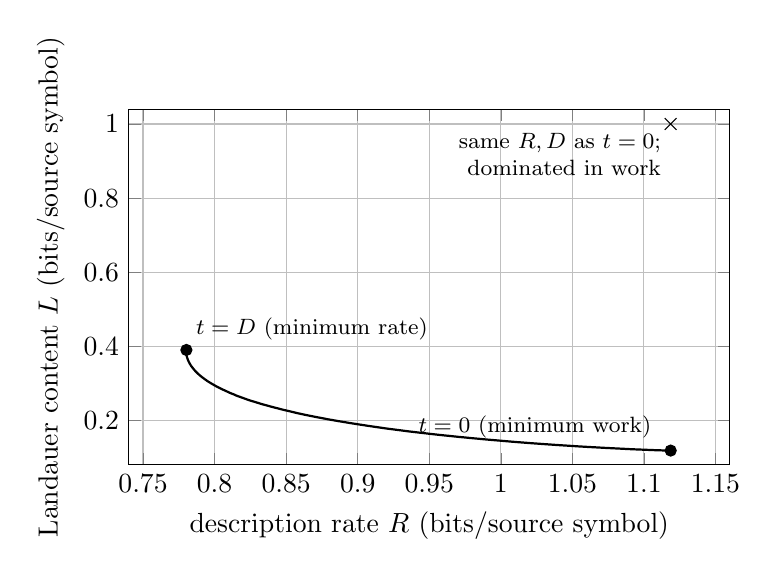
\begin{tikzpicture}
\begin{axis}[
  width=0.76\linewidth,
  height=6.1cm,
  xlabel={description rate $R$ (bits/source symbol)},
  ylabel={Landauer content $L$ (bits/source symbol)},
  xmin=0.74,xmax=1.16,
  ymin=0.08,ymax=1.04,
  grid=major,
  samples=151,
  domain=0.0001:0.15,
  declare function={
    hb(\x)=-(\x*ln(\x)+(1-\x)*ln(1-\x))/ln(2);
  }
]
\addplot[thick,variable=\t]
 ({2-hb(t)-hb(0.30-t)},{1-hb(0.30-t)});
\addplot[only marks,mark=*] coordinates {(1.1187,0.1187) (0.7803,0.3902)};
\node[anchor=south east,font=\footnotesize] at (axis cs:1.112,0.125)
 {$t=0$ (minimum work)};
\node[anchor=south west,font=\footnotesize] at (axis cs:0.7803,0.3902)
 {$t=D$ (minimum rate)};
\addplot[only marks,mark=x,mark size=3pt] coordinates {(1.1187,1.0000)};
\node[anchor=north east,font=\footnotesize,align=right] at (axis cs:1.1187,1.0000)
 {same $R,D$ as $t=0$;\\dominated in work};
\end{axis}
\end{tikzpicture}
\caption{Exact lower rate--work frontier for Proposition~\ref{prop:binary-frontier}
at distortion $D=0.15$. The marked point at $L=1$ comes from reversing the two
component distortions: it has the same rate and source distortion as the
minimum-work endpoint, but about $8.4$ times the Landauer content.}
\label{fig:binary-frontier}
\end{figure}

The matched-rate inversion is immediate. The allocations
$(D_A,D_B)=(0,0.30)$ and $(0.30,0)$ both have
\begin{equation}
 R=2-\hbin(0.30)=1.1187\ \text{bits/source symbol}
\end{equation}
and total distortion $0.15$. Their Landauer contents are respectively
$0.1187$ and $1$ bit/source symbol. The second point is not Pareto optimal, but
it isolates the physical effect: two descriptions tied by ordinary rate and
distortion can differ sharply in reset work.

\section{The materialize-then-project barrier}\label{sec:materialization}

Theorem~\ref{thm:main-region} prices the memory index actually produced by the
observer. It does not say that already recorded information becomes free when a
later computation declares it irrelevant. The next result makes that distinction
exact.

\begin{theorem}[Materialization barrier]\label{thm:materialization}
Suppose a volatile register $A$ first stores the full discrete source block,
$A=X^n$, and a second volatile register stores a deterministic description
$M=f_n(A)$. If both registers are returned to a standard state while $S^n$ is
retained, then their minimum asymptotic ideal reset work is
\begin{equation}
 W_{A,M}^{\star}
 =\kb T\ln2\,H(A,M\mid S^n)
 =n\kb T\ln2\,H(X\mid S).
 \label{eq:materialization-cost}
\end{equation}
This cost is independent of the distortion met by $M$.
\end{theorem}

\begin{proof}
Conditional erasure of the pair $(A,M)$ costs its conditional entropy in the
ideal model. Since $A=X^n$ and $M$ is a function of $A$,
\begin{equation}
 H(A,M\mid S^n)=H(A\mid S^n)=H(X^n\mid S^n)=nH(X\mid S).
\end{equation}
The same result appears under sequential optimal reset. For example,
\begin{equation}
 H(A\mid M,S^n)+H(M\mid S^n)=H(A,M\mid S^n).
\end{equation}
The identity is the chain rule.
\end{proof}

The theorem does not assign a universal work cost to measurement. It says
something narrower: once a complete digital record has been committed to a
volatile logical state, projecting it later cannot refund the work needed to
clear that record. One may retain the discarded detail as reversible garbage
and uncompute it, or avoid recording it. Overwriting it is the irreversible
step.

For a direct consumer-native observer, only $M$ is materialized. Combining
Theorem~\ref{thm:materialization} with Corollary~\ref{cor:cr} gives the ideal
work gap
\begin{equation}
 \Delta W_{\cC}(D,T\mid S)
 =\kb T\ln2\left[H(X\mid S)-L_{\cC}(D\mid S)\right].
 \label{eq:materialization-tax}
\end{equation}
At zero distortion for a deterministic consumer output $U=\cC(X)$,
\begin{equation}
 \Delta W_{\cC}(0,T\mid S)
 =\kb T\ln2\,H(X\mid U,S).
 \label{eq:exact-tax}
\end{equation}
The conditional entropy in \eqref{eq:exact-tax} is the physical price of
materializing distinctions that neither the consumer nor the retained reset
context needs.

This result has an architectural reading. Post-hoc semantic compression can
save communication and downstream storage. It cannot recover the Landauer
saving if a full volatile source record was already created and must be erased.
The thermodynamic advantage requires projection at or before the first digital
memory boundary.

\section{Several consumers}\label{sec:multi}

A practical observer often serves several consumers: a controller, an alarm, an
auditor, and a forensic process may read different functions of the same source.
Let consumer $j$ receive $\widehat X_j^n=g_{j,n}(M)$ and incur distortion
$d_j(X_i,\widehat X_{j,i})$.

\begin{theorem}[Shared observation for several consumers]\label{thm:multi}
For distortion vector $\bm D=(D_1,\ldots,D_m)$, the achievable rate--work region
of one shared memory is
\begin{equation}
\begin{split}
 \RW_{1:m}(\bm D)
 =\clconv\!\bigcup_{p(\hat x_1,\ldots,\hat x_m\mid x)}
 \bigl\{(R,L):\;&R\ge I(X;\widehat X_1,\ldots,\widehat X_m),\\
 &L\ge I(X;\widehat X_1,\ldots,\widehat X_m\mid S)\bigr\},
 \label{eq:multi-region}
\end{split}
\end{equation}
where the union is over joint test channels satisfying
$\E d_j(X,\widehat X_j)\le D_j$ for every $j$.
\end{theorem}

\begin{proof}
Treat the vector reproduction
$\widehat{\bm X}=(\widehat X_1,\ldots,\widehat X_m)$ as the reproduction alphabet
in Theorem~\ref{thm:main-region}. The covering step enforces all $m$ distortion
constraints simultaneously through joint typicality with the vector
reproduction, and the converse applies verbatim with the vector constraint set
in place of $\mathcal T_{\cC}(D)$. Each consumer obtains its component by a
deterministic projection.
\end{proof}

\begin{corollary}[Exact consumers and coordinated reset]\label{cor:tc}
Let $U_j=\cC_j(X)$ be exact deterministic consumer outputs. A joint memory, or
separate memories reset with full cross-memory coordination, has ideal reset
content
\begin{equation}
 H(U_1,\ldots,U_m\mid S).
 \label{eq:joint-exact-work}
\end{equation}
If the $m$ memories are reset independently and each reset sees only $S$, their
contents sum to $\sum_j H(U_j\mid S)$. The excess is the conditional total
correlation
\begin{equation}
 \operatorname{TC}(U_1;\ldots;U_m\mid S)
 =\sum_{j=1}^{m}H(U_j\mid S)-H(U_1,\ldots,U_m\mid S)\ge0.
 \label{eq:conditional-tc}
\end{equation}
\end{corollary}

The qualification about coordinated reset matters. The saving in
\eqref{eq:conditional-tc} is not attached to a particular memory package. It is
obtained whenever the erasure protocol can use the other consumer records as
side information before they are cleared. Independent administrative or
physical reset domains forfeit that correlation.

For observation architecture, the corollary gives a thermodynamic reason to use
a common base representation with consumer-specific refinements. Shared
consumer structure is not merely a compression opportunity; it is conditional
entropy that need not be paid more than once at reset.

\section{Gaussian read geometry, reset side information, and thermal water-filling}\label{sec:gaussian}

The preceding results accept any bounded single-letter distortion. We now
connect them to the local read geometry of Observation Theory. Let
$X\sim\mathcal N(0,\Sigma_X)$ and let a smooth consumer have Jacobian $J_{\cC}$
and output metric $G\succeq0$. Its local read operator is
\begin{equation}
 \PC=J_{\cC}^{\mathsf T}GJ_{\cC}\succeq0,
 \label{eq:readop}
\end{equation}
and the quadratic consumer distortion is
\begin{equation}
 d_{\cC}(x,\hat x)=(x-\hat x)^{\mathsf T}\PC(x-\hat x).
 \label{eq:weighted-dist}
\end{equation}
For a nonlinear consumer, this is the second-order approximation to its output
loss; for a linear consumer with quadratic output loss it is exact
\cite{bond2026observation}.

Let $\lambda_1,\ldots,\lambda_r>0$ be the nonzero eigenvalues of
$\Sigma_X^{1/2}\PC\Sigma_X^{1/2}$, where
$r=\rank(\Sigma_X^{1/2}\PC\Sigma_X^{1/2})$. In an isothermal memory with no
reset side information, rate and Landauer content coincide.

\begin{corollary}[Isothermal read-operator work law]\label{cor:gauss}
For $0<D<\sum_{i=1}^{r}\lambda_i$, let $\theta$ be chosen so that
\begin{equation}
 D=\sum_{i=1}^{r}\min\{\lambda_i,\theta\}.
 \label{eq:water-level}
\end{equation}
Then
\begin{align}
 R_{\cC}(D)=L_{\cC}(D)
 &=\frac12\sum_{i=1}^{r}
 \left[\log_2\frac{\lambda_i}{\theta}\right]_+,
 \label{eq:gaussian-rd}\\
 W_{\cC}^{\star}(D,T)
 &=\frac{\kb T}{2}\sum_{i=1}^{r}
 \left[\ln\frac{\lambda_i}{\theta}\right]_+.
 \label{eq:gaussian-work}
\end{align}
Directions in $\ker\PC$ require neither rate nor reset work, provided they are
never materialized in the observation memory.
\end{corollary}

\begin{proof}
Equation~\eqref{eq:gaussian-rd} is the weighted Gaussian
rate--distortion solution obtained by diagonalizing the read covariance
$\Sigma_X^{1/2}\PC\Sigma_X^{1/2}$ and applying reverse water-filling. Multiply
bits by $\kb T\ln2$ to obtain \eqref{eq:gaussian-work}.
\end{proof}

The final proviso is the materialization barrier in spectral form. A null
read-direction is free to omit. It is not free to erase after it has been
stored.

Reset side information changes the Gaussian picture in a way the scalar case
makes exact.

\begin{proposition}[Scalar Gaussian corner]\label{prop:scalar-corner}
Let $(X,S)$ be jointly Gaussian and zero mean with $\operatorname{Var}X=\sigma^2$
and correlation coefficient $\rho\in(-1,1)$, let
$d(x,\hat x)=(x-\hat x)^2$, and let $0<D<\sigma^2$. Then
\begin{equation}
 \RW(D)
 =\Bigl\{(R,L):
 R\ge\tfrac12\log_2\tfrac{\sigma^2}{D},\
 L\ge\tfrac12\log_2\tfrac{\sigma^2(1-\rho^2)+\rho^2D}{D}
 \Bigr\}.
 \label{eq:scalar-corner}
\end{equation}
Both bounds are attained simultaneously by the classical reverse channel, so
the scalar Gaussian problem has no rate--work tradeoff. The side-information
discount
\begin{equation}
 R_{\min}-L_{\min}
 =\tfrac12\log_2\frac{\sigma^2}{\sigma^2(1-\rho^2)+\rho^2D}
 \label{eq:discount}
\end{equation}
is decreasing in $D$ and increases to $I(X;S)$ as $D\to0$.
\end{proposition}

\begin{proof}
Normalize $\sigma=\sigma_S=1$, and assume $\E\hX=0$ without loss of
generality; centering $\hX$ changes neither mutual information and does not
increase the distortion. Under $\hX-X-S$,
$\E[S\hX]=\E\bigl[\E[S\mid X]\,\E[\hX\mid X]\bigr]=\rho\,\E[X\hX]$, so with
$c=\operatorname{Cov}(X,\hX)$ and $v=\operatorname{Var}\hX\ge c^2$ the second
moments of $(X,\hX,S)$ are determined by $(c,v)$, and the distortion
constraint reads $1-2c+v\le D$; together these force $c>0$ on the feasible
set. For the work coordinate,
$L=h(X\mid S)-h(X\mid\hX,S)$ and
$h(X\mid\hX,S)\le\tfrac12\log2\pi e\,e_{\mathrm{lin}}$, where
$e_{\mathrm{lin}}$ is the error of the best linear estimate of $X$ from
$(\hX,S)$; the bound holds for any reproduction alphabet, discrete included.
A direct computation gives
$e_{\mathrm{lin}}=(1-\rho^2)(v-c^2)/(v-\rho^2c^2)$, hence
\begin{equation}
 L\ \ge\ \tfrac12\log_2\frac{v-\rho^2c^2}{v-c^2}.
 \label{eq:moment-bound}
\end{equation}
The right side of \eqref{eq:moment-bound} decreases in $v$, so the distortion
constraint binds, $v=D-1+2c$. On that line the stationarity condition of the
ratio reduces to $(1-\rho^2)\,c\,(c+D-1)=0$; the root $c=0$ is infeasible,
the interior point $c=1-D$ has positive second derivative, the boundary
values diverge, and the minimum is $(1-\rho^2+\rho^2D)/D$. The
rate converse is classical. The reverse channel $\hX=(1-D)X+W$ with
$W\sim\mathcal N(0,D(1-D))$ independent of $(X,S)$ has $c=v=1-D$, distortion
exactly $D$, and attains both bounds, so the region is the stated quadrant.
Monotonicity of \eqref{eq:discount} and the limit
$\tfrac12\log_2\frac1{1-\rho^2}=I(X;S)$ are elementary.
\end{proof}

Within the jointly Gaussian family, $L$ is in fact a function of $R$ alone,
$L=\tfrac12\log_2\!\bigl(1+(1-\rho^2)(2^{2R}-1)\bigr)$; a scalar source
offers no allocation freedom. The binary frontier of
Proposition~\ref{prop:binary-frontier} came from allocating distortion
between a component the reset context knows and one it does not. The next
proposition restores exactly that mechanism.

\begin{proposition}[Vector frontier and reset water-filling]\label{prop:vector-frontier}
Let $X$ have independent components $X_i\sim\mathcal N(0,\sigma_i^2)$,
$i=1,\ldots,r$, let $S=(S_1,\ldots,S_r)$ with $S_i$ jointly Gaussian with
$X_i$ alone at correlation $\rho_i$, and let
$d(x,\hat x)=\sum_i p_i(x_i-\hat x_i)^2$ with $p_i>0$, the read geometry of
\eqref{eq:weighted-dist} with independently read and independently known
modes. Write $c_i=\sigma_i^2(1-\rho_i^2)$. The lower Pareto boundary of
$\RW(D)$ is traced by $\alpha\in[0,1]$ as follows. With $\mu>0$ chosen so
that $\sum_i p_id_i=D$, allocate $d_i=\min\{\sigma_i^2,\delta_i(\mu)\}$,
where $\delta_i(\mu)$ is the positive root of
\begin{equation}
 2\mu p_i\rho_i^2\,\delta^2
 +\bigl(2\mu p_ic_i-\alpha\rho_i^2\bigr)\,\delta
 -c_i=0
 \label{eq:alloc-quadratic}
\end{equation}
and $\delta_i=1/(2\mu p_i)$ when $\rho_i=0$; the frontier point is
\begin{equation}
 R=\sum_{i=1}^{r}\tfrac12\log_2\frac{\sigma_i^2}{d_i},
 \qquad
 L=\sum_{i=1}^{r}\tfrac12\log_2\frac{c_i+\rho_i^2d_i}{d_i}.
 \label{eq:vector-frontier}
\end{equation}
At $\alpha=1$ the rule is classical reverse water-filling. At $\alpha=0$ it
allocates distortion toward the modes the reset context knows least. A mode
with $d_i=\sigma_i^2$ contributes zero to both coordinates.
\end{proposition}

\begin{proof}
For independent pairs $(X_i,S_i)$ and any code with $\hX-X-S$, the
componentwise analogue of Appendix~\ref{app:converse} gives
$I(X;\hX)\ge\sum_iI(X_i;\hX_i)$ and
$I(X;\hX\mid S)\ge\sum_iI(X_i;\hX_i\mid S_i)$.
Proposition~\ref{prop:scalar-corner} bounds each mode at its own distortion
$d_i=\E(X_i-\hX_i)^2$, so every achievable pair is dominated by the
allocation program that minimizes
$\alpha\sum_iR_i(d_i)+(1-\alpha)\sum_iL_i(d_i)$ over
$\sum_ip_id_i\le D$, $0<d_i\le\sigma_i^2$. Each $R_i$ is convex in $d_i$, and
\begin{equation*}
 L_i''(d)\ \propto\ \frac1{d^2}-\frac{\rho_i^4}{(c_i+\rho_i^2d)^2}\ >\ 0
 \quad\text{exactly when } c_i>0,
\end{equation*}
so the program is convex and its KKT condition
\begin{equation}
 \frac{\alpha}{2d_i}
 +\frac{(1-\alpha)\,c_i}{2d_i\bigl(c_i+\rho_i^2d_i\bigr)}
 =\mu p_i
 \label{eq:alloc-kkt}
\end{equation}
is sufficient; clearing denominators gives \eqref{eq:alloc-quadratic}.
Products of scalar reverse channels achieve every allocation, convexity of
the per-mode objectives makes the achievable set convex, and the weighted-sum
sweep therefore traces the entire lower boundary; strict convexity makes the
minimizer unique at every $\alpha$, endpoints included. The last claim is the
identity $c_i+\rho_i^2\sigma_i^2=\sigma_i^2$.
\end{proof}

Setting every $\rho_i=0$ gives $L\equiv R$ and recovers
Corollary~\ref{cor:gauss}. The tradeoff lives entirely in the heterogeneity
of the $\rho_i$ and $\sigma_i$. For two unit-variance modes with
$\rho=(0.95,0)$, equal read weights, and $D=0.5$, the minimum-rate and
minimum-work allocations differ by about $0.11$ bits of Landauer content and
$0.13$ bits of rate at matched distortion; the reproducibility materials
carry the exact frontier. This is the Gaussian analogue of the binary
frontier, with the water level of \eqref{eq:alloc-kkt} playing the role of
the allocation parameter $t$.

The Landauer scale also changes the allocation rule when different components
of the observation are reset against different reservoirs. Consider physically
separate memory banks, with eigenmode $i$ reset at temperature $T_i>0$. Let
$d_i\le\lambda_i$ be its allocated distortion. Independent Gaussian coding
requires $r_i=\frac12\log_2(\lambda_i/d_i)$ bits for an active mode and costs
$\kb T_i\ln2\,r_i$ of ideal reset work.

\begin{proposition}[Temperature-weighted water-filling]\label{prop:thermal-waterfill}
Under the independent eigenmode memory model, the minimum ideal reset work at
total distortion $D$ is attained by
\begin{equation}
 d_i^{\star}=\min\{\lambda_i,\nu T_i\},
 \qquad
 \sum_{i=1}^{r}d_i^{\star}=D,
 \label{eq:thermal-d}
\end{equation}
for a unique $\nu>0$ in the nontrivial range. The minimum work is
\begin{equation}
 \boxed{
 W_{\mathrm{het}}^{\star}(D)
 =\frac{\kb}{2}\sum_{i=1}^{r}T_i
 \left[\ln\frac{\lambda_i}{\nu T_i}\right]_+.}
 \label{eq:thermal-waterfill}
\end{equation}
When all $T_i$ are equal, \eqref{eq:thermal-d} reduces to ordinary reverse
water-filling.
\end{proposition}

\begin{proof}
For active mode $i$,
\begin{equation}
 W_i(d_i)=\frac{\kb T_i}{2}\ln\frac{\lambda_i}{d_i}.
\end{equation}
Minimize $\sum_i W_i(d_i)$ subject to
$0<d_i\le\lambda_i$ and $\sum_i d_i\le D$. The KKT stationarity condition for
an active mode is
\begin{equation}
 -\frac{\kb T_i}{2d_i}+\mu=0,
\end{equation}
so $d_i=(\kb/2\mu)T_i=\nu T_i$. Clipping at $\lambda_i$ gives
\eqref{eq:thermal-d}; substitution gives \eqref{eq:thermal-waterfill}.
\end{proof}

The rule allocates more distortion to modes stored in hotter banks. This is not
a claim about one isothermal register. It is a design result for a physically
partitioned observer whose reset environments have different marginal work per
bit.

\section{Staleness as lost relevance and increased reset work}\label{sec:stale}

Side information at reset need not be a static auxiliary variable. It may be a
later state of the process that generated the record. This produces a simple
link between age, relevance, and work.

\begin{proposition}[Staleness-work complement]\label{prop:stale}
Let $X_0,X_1,\ldots$ be a stationary Markov chain, and let a stored record $M$
be generated from $X_0$, so that $M$ is conditionally independent of the future
trajectory $(X_1,X_2,\ldots)$ given $X_0$. If $X_t$ is retained when $M$ is
erased, then the ideal Landauer content at age $t$ is
\begin{equation}
 L_t=H(M\mid X_t)=H(M)-I(M;X_t).
 \label{eq:stale-complement}
\end{equation}
Moreover, $L_t$ is nondecreasing in $t$.
\end{proposition}

\begin{proof}
The identity is the definition of mutual information. Under the hypothesis the
joint law factors as $p(x_0)\,p(m\mid x_0)\,p(x_t\mid x_0)\,p(x_{t+1}\mid x_t)$,
from which $p(x_{t+1}\mid x_t,m)=p(x_{t+1}\mid x_t)$: the chain
$M-X_t-X_{t+1}$ is Markov. Data processing then gives
$I(M;X_{t+1})\le I(M;X_t)$, hence the monotonicity of $L_t$.
\end{proof}

The unconditional reset cost $H(M)$ has not changed. What changes is the share
of that cost that can be reversibly discharged by correlation with the current
state. An old record is less useful for predicting the present and, for exactly
the same reason, harder to erase using the present as side information.

\begin{example}[Symmetric binary Markov record]\label{ex:markov}
Let $X_t$ be a stationary fair bit that flips independently with probability
$p\in(0,1/2)$ per step, and store $M=X_0$. At age $t$,
\begin{equation}
 q_t=\Pr\{X_t\ne X_0\}
 =\frac{1-(1-2p)^t}{2}.
 \label{eq:q-age}
\end{equation}
Therefore
\begin{align}
 I(X_0;X_t)&=1-\hbin(q_t),\label{eq:predictive-age}\\
 L_t=H(X_0\mid X_t)&=\hbin(q_t),\label{eq:work-age}
\end{align}
so predictive information and conditional reset content sum to one bit for
every age. Figure~\ref{fig:stale} shows the exchange for $p=0.05$.
\end{example}

\begin{figure}[!t]
\centering
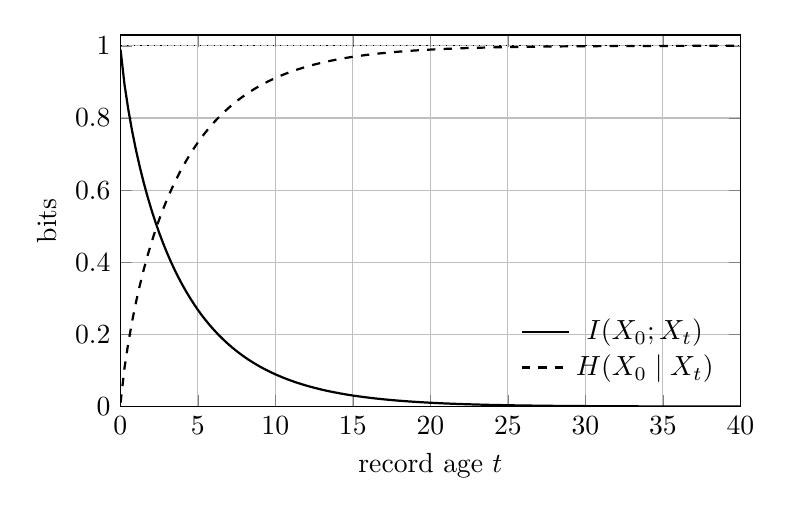
\begin{tikzpicture}
\begin{axis}[
  width=0.78\linewidth,
  height=6.3cm,
  xlabel={record age $t$},
  ylabel={bits},
  xmin=0,xmax=40,
  ymin=0,ymax=1.03,
  grid=major,
  legend style={at={(0.98,0.04)},anchor=south east,draw=none,fill=none},
  samples=161,
  domain=0.02:40,
  declare function={
    qage(\x)=0.5*(1-pow(0.9,\x));
    hb(\x)=-(\x*ln(\x)+(1-\x)*ln(1-\x))/ln(2);
  }
]
\addplot[thick] {1-hb(qage(x))};
\addplot[thick,forget plot] coordinates {(0,1)};
\addlegendentry{$I(X_0;X_t)$}
\addplot[thick,dashed] {hb(qage(x))};
\addplot[thick,dashed,forget plot] coordinates {(0,0)};
\addlegendentry{$H(X_0\mid X_t)$}
\addplot[thin,dotted] {1};
\end{axis}
\end{tikzpicture}
\caption{For a symmetric binary Markov source with $p=0.05$, predictive
information lost with age is gained exactly as conditional Landauer content.
The unconditional content of the stored fair bit remains one bit.}
\label{fig:stale}
\end{figure}

The correlation law $(1-2p)^t$ often appears as a value-of-information decay.
Equations~\eqref{eq:predictive-age}--\eqref{eq:work-age} give it a second
interpretation: age transfers one fixed bit from side-information-assisted
reversibility into unavoidable reset uncertainty.

\section{Relation to prior work}\label{sec:prior}

Landauer identified logical irreversibility with unavoidable heat generation
in physical computation \cite{landauer1961}; Bennett showed that arbitrary
computation can be embedded in a logically reversible process, postponing the
cost to the erasure of retained history \cite{bennett1973}. Later work placed
measurement and erasure in explicit thermodynamic accounting frameworks
\cite{sagawa2009,parrondo2015}. Del Rio \emph{et al.} showed that erasure work
is governed by entropy conditioned on an observer's side information
\cite{delrio2011}. Faist \emph{et al.} characterized the work cost of a general
logical process through information discarded conditional on its output
\cite{faist2015}. In an algorithmic, single-string setting, Zurek identified
the thermodynamic cost of erasing a record with its compressed length
\cite{zurek1989}, and Wolf sharpened the erasure principle to the
compressibility of the string given the erasing agent's knowledge
\cite{wolf2018}. The present paper is a block-coding, lossy, and
consumer-constrained counterpart of that observation: the object whose
conditional compressibility is priced is a description that must remain
decodable by a consumer lacking the side information available at reset.
These results supply the physical accounting used here; this paper does not
alter Landauer's principle (Remark~\ref{rem:invariance}).

On the source-coding side, Shannon's fidelity-constrained coding theorem
introduced the rate--distortion function \cite{shannon1959}. Wyner and Ziv
characterized lossy coding when side information is available only at the
decoder \cite{wynerziv1976}. Steinberg imposed common reconstruction, requiring
the reproduction to be determined without relying on decoder-only side
information \cite{steinberg2009}. Equation~\eqref{eq:work-endpoint} is exactly
that common-reconstruction functional.

The distinction between codebook size and output entropy is also classical.
Entropy-constrained vector quantization replaces a fixed-rate objective by the
entropy of the quantizer output \cite{chou1989}; conditional
entropy-constrained quantization exploits a retained context when coding a
sequence of quantizer outputs \cite{chou1990}. Those works are an important
precursor to the two-resource view. Theorem~\ref{thm:main-region} differs in
holding the full fixed description available to a consumer that lacks $S$ while
pricing the conditional entropy left for a separate reset mechanism that has
$S$. Its thermodynamic content depends on that lifecycle distinction, not on the
claim that output entropy had previously been ignored.

A second neighboring line relates thermodynamic efficiency to rate--distortion,
relevance, and prediction. Still derived the rate--distortion objective from a
least-effort principle for preparing a representation \cite{still2014lossy}.
Still \emph{et al.} then identified nonpredictive information as a lower bound on
dissipation in driven systems \cite{still2012}; subsequent work showed that
retaining irrelevant memory limits thermodynamic efficiency and connects an
information engine to the information bottleneck \cite{still2020}. The present
model prices a different stage of the cycle: conditional reset of an already
available description. Relevance is specified by an arbitrary consumer
distortion rather than only future prediction; the description must remain
decodable without the reset side information; and the main object is a joint
rate--work region rather than a single preparation or dissipation bound.

Observation Theory supplies the consumer geometry used in
Section~\ref{sec:gaussian}: a consumer pulls its output metric back to a positive
semidefinite read operator, and the resulting distortion defines a
consumer-relative rate--distortion problem \cite{bond2026observation}. The
present paper starts after that geometry has been identified. It asks which
parts of the resulting representation must be erased, under which retained
correlations, and at what ideal work.

\section{Limits and extensions}\label{sec:limits}

Several extensions are natural, but they require a different physical or
information-theoretic model.

\emph{Conditional entropy coding.} The physical interpretation in this paper
sits beside a substantial literature on entropy-constrained and conditional
entropy-constrained quantization. The single-letter region above is stated for
asymptotically long memoryless blocks; finite-dimensional quantizer structure,
causal conditioning contexts, and implementable conditional reset circuits are
separate design problems.


\emph{Finite blocklength and one-shot work.} The proof uses typicality and
asymptotic conditional entropy. At finite $n$, smooth max-entropies and error
budgets replace Shannon entropy in the most general work bounds
\cite{faist2015}. A second-order rate--work region would have two dispersions and
need not be obtained by simply scaling a finite-blocklength rate--distortion
formula.

\emph{Nondegenerate memories and finite time.} If logical states have different
energies, free-energy differences enter the accounting. If reset must finish in
finite time or under time-symmetric controls, additional dissipation can dominate
the Landauer term \cite{reeb2014}. Proposition~\ref{prop:thermal-waterfill}
allows different bath temperatures but retains degenerate logical memories and
quasistatic reset.

\emph{Quantum side information.} Conditional quantum entropy can be negative,
allowing work extraction during erasure \cite{delrio2011}. The rate coordinate
would then have to be coupled to a quantum source-coding model. Nothing in
Theorem~\ref{thm:main-region} should be read as a quantum characterization.

\emph{Side information acquisition.} The reset context $S^n$ is assumed to
survive for free. If it must itself be sensed, stored, transmitted, or erased,
its lifecycle belongs in the optimization. A rate-limited erasure helper would
produce a three-memory problem rather than the two-coordinate region studied
here.

\emph{General Gaussian coupling.} Proposition~\ref{prop:vector-frontier}
assumes independently read and independently known modes. When $\Sigma_X$,
$\Sigma_{X\mid S}$, and $\PC$ are not simultaneously diagonalizable, the
allocation program becomes a joint semidefinite optimization and the frontier
need not separate across modes; its characterization is left open.

\emph{Sources with memory.} Proposition~\ref{prop:stale} uses memory directly,
but the coding theorem is i.i.d. Information-spectrum methods should extend the
region to general sources, with conditional spectral information rates replacing
single-letter mutual informations.

\section{Conclusion}\label{sec:conclusion}

A useful observation is not only a message. It is a physical memory state with
a lifecycle. Theorem~\ref{thm:main-region} separates two costs of that state:
the information a consumer must receive and the uncertainty a reset mechanism
must irreversibly discard. Side information available only at reset can lower
the second cost without helping the consumer with the first.

The distinction sharpens consumer-relative observation. The consumer determines
which source distinctions must survive distortion. The reset context determines
which of the stored distinctions remain predictable when the memory is cleared.
The binary frontier shows why neither coordinate can be inferred from the
other: a code that minimizes description capacity need not minimize reset work.
Landauer's principle then prices the residue. In the exact case, that residue is
$H(\cC(X)\mid S)$. In the Gaussian local model, it is the ordinary read-operator
water-filling rate multiplied by $\kb T\ln2$. Across several consumers, it is the
conditional entropy of their joint read rather than the sum of isolated records.

The materialization theorem states the practical boundary most plainly. Once a
full volatile source record exists, later projection cannot make its erasure
cheap. A consumer-relative observer reaches the lower work law only by avoiding
that record, or by preserving enough reversible history to uncompute it. The
thermodynamic consequence of Observation Theory is therefore not that irrelevant
information disappears. It is that an observer should decide what is irrelevant
before turning it into a bit that must later be erased.

\appendices

\section{Single-letter converse details}\label{app:converse}

For completeness, we justify the last inequalities in
\eqref{eq:rate-conv} and \eqref{eq:work-conv}. For the rate coordinate,
\begin{align}
 I(X^n;\hXn)
 &=H(X^n)-H(X^n\mid\hXn)\nonumber\\
 &=\sum_{i=1}^{n}H(X_i)
   -\sum_{i=1}^{n}H(X_i\mid X^{i-1},\hXn)\nonumber\\
 &\ge\sum_{i=1}^{n}\left[H(X_i)-H(X_i\mid\hX_i)\right]\nonumber\\
 &=\sum_{i=1}^{n}I(X_i;\hX_i).
\end{align}
For the work coordinate,
\begin{align}
 I(X^n;\hXn\mid S^n)
 &=H(X^n\mid S^n)-H(X^n\mid\hXn,S^n)\nonumber\\
 &=\sum_{i=1}^{n}H(X_i\mid S_i)
   -\sum_{i=1}^{n}H(X_i\mid X^{i-1},\hXn,S^n)\nonumber\\
 &\ge\sum_{i=1}^{n}
 \left[H(X_i\mid S_i)-H(X_i\mid\hX_i,S_i)\right]\nonumber\\
 &=\sum_{i=1}^{n}I(X_i;\hX_i\mid S_i).
\end{align}

\bibliographystyle{IEEEtran}
\bibliography{consumer-relative-landauer}

\end{document}
